\documentclass{beamer}
%\usetheme{lankton-keynote}
%\usetheme{Gombak} ni cerah
\usetheme{Ampang}% ni gelap

\usepackage{ubuntu}
\usepackage{beamerthemesplitku}

%\usepackage{beamerthemetree}
%\usecolortheme{beaver}
\usecolortheme{ampangcolor}
%\usecolortheme{warna}
\usepackage{graphicx}
\usepackage{tikz}
\usepackage{forest}
\usetikzlibrary{arrows,shapes,positioning,shadows,trees}

%\newtheorem{algorithm}{Algorithm}[section] 
\usepackage{float}
\floatstyle{ruled}


\usepackage{fancyvrb}
\usepackage{tabularx}
\usepackage{graphicx}
\usepackage{longtable}
%\usepackage{ccaption} 
\usepackage{listings}

\usepackage{color}

%\setbeamercolor{frametitle}{black!100,fg=white}
%\setbeamercolor{titlelike}{parent=structure,bg=red!60!blue!90!green!95,fg=white}
%\setbeamercolor*{palette primary}{use=structure,bg=red!60!blue!90!green!95,fg=white}
%\setbeamercolor*{palette quaternary}{use=structure,bg=red!10!black!100,fg=white}


\makeatletter
\def\PY@reset{\let\PY@it=\relax \let\PY@bf=\relax%
    \let\PY@ul=\relax \let\PY@tc=\relax%
    \let\PY@bc=\relax \let\PY@ff=\relax}
\def\PY@tok#1{\csname PY@tok@#1\endcsname}
\def\PY@toks#1+{\ifx\relax#1\empty\else%
    \PY@tok{#1}\expandafter\PY@toks\fi}
\def\PY@do#1{\PY@bc{\PY@tc{\PY@ul{%
    \PY@it{\PY@bf{\PY@ff{#1}}}}}}}
\def\PY#1#2{\PY@reset\PY@toks#1+\relax+\PY@do{#2}}

\expandafter\def\csname PY@tok@gd\endcsname{\def\PY@tc##1{\textcolor[rgb]{0.63,0.00,0.00}{##1}}}
\expandafter\def\csname PY@tok@gu\endcsname{\let\PY@bf=\textbf\def\PY@tc##1{\textcolor[rgb]{0.50,0.00,0.50}{##1}}}
\expandafter\def\csname PY@tok@gt\endcsname{\def\PY@tc##1{\textcolor[rgb]{0.00,0.27,0.87}{##1}}}
\expandafter\def\csname PY@tok@gs\endcsname{\let\PY@bf=\textbf}
\expandafter\def\csname PY@tok@gr\endcsname{\def\PY@tc##1{\textcolor[rgb]{1.00,0.00,0.00}{##1}}}
\expandafter\def\csname PY@tok@cm\endcsname{\let\PY@it=\textit\def\PY@tc##1{\textcolor[rgb]{0.25,0.50,0.50}{##1}}}
\expandafter\def\csname PY@tok@vg\endcsname{\def\PY@tc##1{\textcolor[rgb]{0.10,0.09,0.49}{##1}}}
\expandafter\def\csname PY@tok@m\endcsname{\def\PY@tc##1{\textcolor[rgb]{0.40,0.40,0.40}{##1}}}
\expandafter\def\csname PY@tok@mh\endcsname{\def\PY@tc##1{\textcolor[rgb]{0.40,0.40,0.40}{##1}}}
\expandafter\def\csname PY@tok@go\endcsname{\def\PY@tc##1{\textcolor[rgb]{0.53,0.53,0.53}{##1}}}
\expandafter\def\csname PY@tok@ge\endcsname{\let\PY@it=\textit}
\expandafter\def\csname PY@tok@vc\endcsname{\def\PY@tc##1{\textcolor[rgb]{0.10,0.09,0.49}{##1}}}
\expandafter\def\csname PY@tok@il\endcsname{\def\PY@tc##1{\textcolor[rgb]{0.40,0.40,0.40}{##1}}}
\expandafter\def\csname PY@tok@cs\endcsname{\let\PY@it=\textit\def\PY@tc##1{\textcolor[rgb]{0.25,0.50,0.50}{##1}}}
\expandafter\def\csname PY@tok@cp\endcsname{\def\PY@tc##1{\textcolor[rgb]{0.74,0.48,0.00}{##1}}}
\expandafter\def\csname PY@tok@gi\endcsname{\def\PY@tc##1{\textcolor[rgb]{0.00,0.63,0.00}{##1}}}
\expandafter\def\csname PY@tok@gh\endcsname{\let\PY@bf=\textbf\def\PY@tc##1{\textcolor[rgb]{0.00,0.00,0.50}{##1}}}
\expandafter\def\csname PY@tok@ni\endcsname{\let\PY@bf=\textbf\def\PY@tc##1{\textcolor[rgb]{0.60,0.60,0.60}{##1}}}
\expandafter\def\csname PY@tok@nl\endcsname{\def\PY@tc##1{\textcolor[rgb]{0.63,0.63,0.00}{##1}}}
\expandafter\def\csname PY@tok@nn\endcsname{\let\PY@bf=\textbf\def\PY@tc##1{\textcolor[rgb]{0.00,0.00,1.00}{##1}}}
\expandafter\def\csname PY@tok@no\endcsname{\def\PY@tc##1{\textcolor[rgb]{0.53,0.00,0.00}{##1}}}
\expandafter\def\csname PY@tok@na\endcsname{\def\PY@tc##1{\textcolor[rgb]{0.49,0.56,0.16}{##1}}}
\expandafter\def\csname PY@tok@nb\endcsname{\def\PY@tc##1{\textcolor[rgb]{0.00,0.50,0.00}{##1}}}
\expandafter\def\csname PY@tok@nc\endcsname{\let\PY@bf=\textbf\def\PY@tc##1{\textcolor[rgb]{0.00,0.00,1.00}{##1}}}
\expandafter\def\csname PY@tok@nd\endcsname{\def\PY@tc##1{\textcolor[rgb]{0.67,0.13,1.00}{##1}}}
\expandafter\def\csname PY@tok@ne\endcsname{\let\PY@bf=\textbf\def\PY@tc##1{\textcolor[rgb]{0.82,0.25,0.23}{##1}}}
\expandafter\def\csname PY@tok@nf\endcsname{\def\PY@tc##1{\textcolor[rgb]{0.00,0.00,1.00}{##1}}}
\expandafter\def\csname PY@tok@si\endcsname{\let\PY@bf=\textbf\def\PY@tc##1{\textcolor[rgb]{0.73,0.40,0.53}{##1}}}
\expandafter\def\csname PY@tok@s2\endcsname{\def\PY@tc##1{\textcolor[rgb]{0.73,0.13,0.13}{##1}}}
\expandafter\def\csname PY@tok@vi\endcsname{\def\PY@tc##1{\textcolor[rgb]{0.10,0.09,0.49}{##1}}}
\expandafter\def\csname PY@tok@nt\endcsname{\let\PY@bf=\textbf\def\PY@tc##1{\textcolor[rgb]{0.00,0.50,0.00}{##1}}}
\expandafter\def\csname PY@tok@nv\endcsname{\def\PY@tc##1{\textcolor[rgb]{0.10,0.09,0.49}{##1}}}
\expandafter\def\csname PY@tok@s1\endcsname{\def\PY@tc##1{\textcolor[rgb]{0.73,0.13,0.13}{##1}}}
\expandafter\def\csname PY@tok@sh\endcsname{\def\PY@tc##1{\textcolor[rgb]{0.73,0.13,0.13}{##1}}}
\expandafter\def\csname PY@tok@sc\endcsname{\def\PY@tc##1{\textcolor[rgb]{0.73,0.13,0.13}{##1}}}
\expandafter\def\csname PY@tok@sx\endcsname{\def\PY@tc##1{\textcolor[rgb]{0.00,0.50,0.00}{##1}}}
\expandafter\def\csname PY@tok@bp\endcsname{\def\PY@tc##1{\textcolor[rgb]{0.00,0.50,0.00}{##1}}}
\expandafter\def\csname PY@tok@c1\endcsname{\let\PY@it=\textit\def\PY@tc##1{\textcolor[rgb]{0.25,0.50,0.50}{##1}}}
\expandafter\def\csname PY@tok@kc\endcsname{\let\PY@bf=\textbf\def\PY@tc##1{\textcolor[rgb]{0.00,0.50,0.00}{##1}}}
\expandafter\def\csname PY@tok@c\endcsname{\let\PY@it=\textit\def\PY@tc##1{\textcolor[rgb]{0.25,0.50,0.50}{##1}}}
\expandafter\def\csname PY@tok@mf\endcsname{\def\PY@tc##1{\textcolor[rgb]{0.40,0.40,0.40}{##1}}}
\expandafter\def\csname PY@tok@err\endcsname{\def\PY@bc##1{\setlength{\fboxsep}{0pt}\fcolorbox[rgb]{1.00,0.00,0.00}{1,1,1}{\strut ##1}}}
\expandafter\def\csname PY@tok@kd\endcsname{\let\PY@bf=\textbf\def\PY@tc##1{\textcolor[rgb]{0.00,0.50,0.00}{##1}}}
\expandafter\def\csname PY@tok@ss\endcsname{\def\PY@tc##1{\textcolor[rgb]{0.10,0.09,0.49}{##1}}}
\expandafter\def\csname PY@tok@sr\endcsname{\def\PY@tc##1{\textcolor[rgb]{0.73,0.40,0.53}{##1}}}
\expandafter\def\csname PY@tok@mo\endcsname{\def\PY@tc##1{\textcolor[rgb]{0.40,0.40,0.40}{##1}}}
\expandafter\def\csname PY@tok@kn\endcsname{\let\PY@bf=\textbf\def\PY@tc##1{\textcolor[rgb]{0.00,0.50,0.00}{##1}}}
\expandafter\def\csname PY@tok@mi\endcsname{\def\PY@tc##1{\textcolor[rgb]{0.40,0.40,0.40}{##1}}}
\expandafter\def\csname PY@tok@gp\endcsname{\let\PY@bf=\textbf\def\PY@tc##1{\textcolor[rgb]{0.00,0.00,0.50}{##1}}}
\expandafter\def\csname PY@tok@o\endcsname{\def\PY@tc##1{\textcolor[rgb]{0.40,0.40,0.40}{##1}}}
\expandafter\def\csname PY@tok@kr\endcsname{\let\PY@bf=\textbf\def\PY@tc##1{\textcolor[rgb]{0.00,0.50,0.00}{##1}}}
\expandafter\def\csname PY@tok@s\endcsname{\def\PY@tc##1{\textcolor[rgb]{0.73,0.13,0.13}{##1}}}
\expandafter\def\csname PY@tok@kp\endcsname{\def\PY@tc##1{\textcolor[rgb]{0.00,0.50,0.00}{##1}}}
\expandafter\def\csname PY@tok@w\endcsname{\def\PY@tc##1{\textcolor[rgb]{0.73,0.73,0.73}{##1}}}
\expandafter\def\csname PY@tok@kt\endcsname{\def\PY@tc##1{\textcolor[rgb]{0.69,0.00,0.25}{##1}}}
\expandafter\def\csname PY@tok@ow\endcsname{\let\PY@bf=\textbf\def\PY@tc##1{\textcolor[rgb]{0.67,0.13,1.00}{##1}}}
\expandafter\def\csname PY@tok@sb\endcsname{\def\PY@tc##1{\textcolor[rgb]{0.73,0.13,0.13}{##1}}}
\expandafter\def\csname PY@tok@k\endcsname{\let\PY@bf=\textbf\def\PY@tc##1{\textcolor[rgb]{0.00,0.50,0.00}{##1}}}
\expandafter\def\csname PY@tok@se\endcsname{\let\PY@bf=\textbf\def\PY@tc##1{\textcolor[rgb]{0.73,0.40,0.13}{##1}}}
\expandafter\def\csname PY@tok@sd\endcsname{\let\PY@it=\textit\def\PY@tc##1{\textcolor[rgb]{0.73,0.13,0.13}{##1}}}

\def\PYZbs{\char`\\}
\def\PYZus{\char`\_}
\def\PYZob{\char`\{}
\def\PYZcb{\char`\}}
\def\PYZca{\char`\^}
\def\PYZam{\char`\&}
\def\PYZlt{\char`\<}
\def\PYZgt{\char`\>}
\def\PYZsh{\char`\#}
\def\PYZpc{\char`\%}
\def\PYZdl{\char`\$}
\def\PYZhy{\char`\-}
\def\PYZsq{\char`\'}
\def\PYZdq{\char`\"}
\def\PYZti{\char`\~}
% for compatibility with earlier versions
\def\PYZat{@}
\def\PYZlb{[}
\def\PYZrb{]}
\makeatother




\setbeamertemplate{navigation symbols}{} %no nav symbols
%\logo{\includegraphics[width=12.6cm,height=1cm]{kul.png}}
\logo{
\includegraphics[scale=0.2]{mosc.jpg}}
%\logo{\includegraphics[scale=0.15]{cambridge.png}}
\title[MOSC 2014\hspace{2em}\insertframenumber/\inserttotalframenumber]{\fontUbuntuCondensed Android Custom Kernel/ROM design}
\author[Muhammad Najmi]{Muhammad Najmi Ahmad Zabidi\\
[1.7ex]\tiny{\textit{IIUM}}}
\institute{MOSC 2014\\Menara SSM \\ Kuala Lumpur, Malaysia}
%\institute{FSKSM, UTM Skudai, JB}

\date{24-25 September 2014}

\begin{document} 
\setbeamerfont{frametitle}{size=\small}
\maketitle

\lstset{basicstyle=\ttfamily\tiny}

\begin{frame}{About}
 \begin{itemize}
  \item I am a research grad student in Universiti Teknologi Malaysia, Skudai, Johor Bahru, Malaysia
  \item My current employer is International Islamic University Malaysia, Kuala Lumpur
  \item Research area - malware detection, narrowing on Windows executables
  \item Doing things on Android kernel and ROM due to some stories...
 \end{itemize}

\end{frame}

\begin{frame}{A bit about Android}

\begin{columns}[t]
 \begin{column}{5cm}
  
 
\includegraphics[scale=0.35]{linux-android.jpg}
 
 
 \end{column}


\begin{column}{5cm}
 
 
 \begin{itemize}
  \item Android is a mobile operating system
  \item Using \emph{Linux} kernel
  \item Components for kernel are C language
  \item Components for interface are mostly C++ and Java
 \end{itemize}

 
\end{column}

 \end{columns}
 
\end{frame}




\begin{frame}{Comparison between Android kernel and ROM}

\begin{table}
 \begin{tabular} { p{5cm}| p{5cm} }
 \hline\hline
  Kernel&ROM\\
  \hline
  
  GPL licensed & Apache licensed\\
  \hline
  
  Source code must be published & Source code is not compulsory to be published.
  Hence any modifications are not neccessarily going back to the public\\
  
  \hline
  
 \end{tabular}

\end{table}
\end{frame}


\begin{frame}{Android structure}
 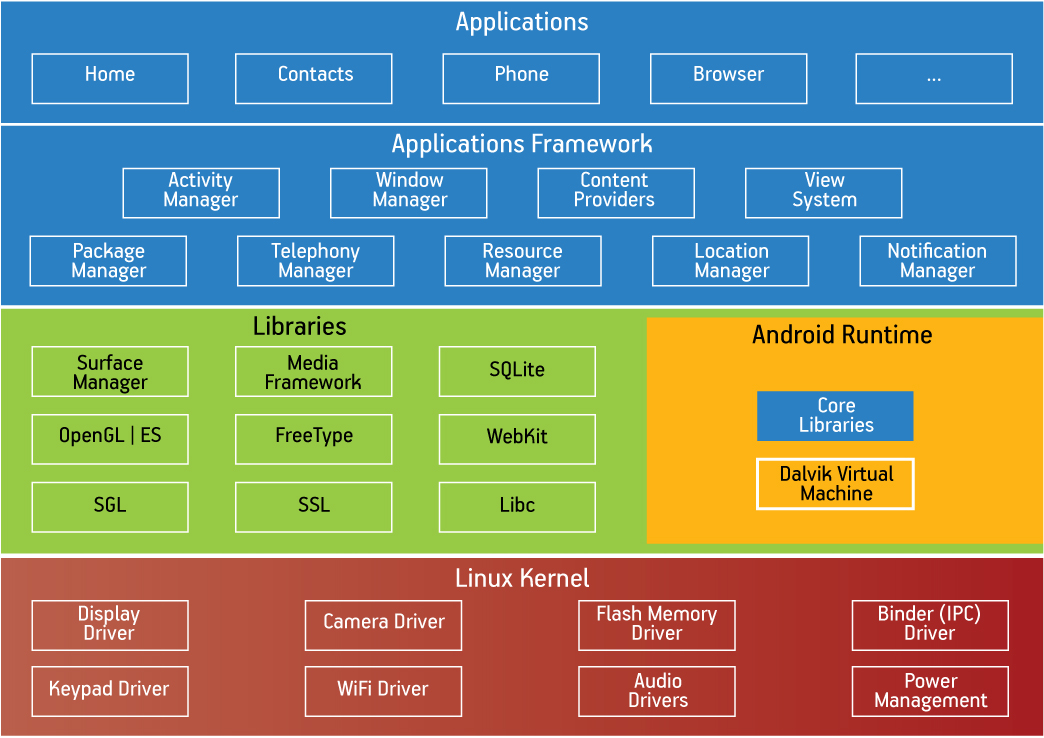
\includegraphics[scale=0.3]{android.jpg}
\end{frame}


\begin{frame}{Android kernel vs Linux kernel}
 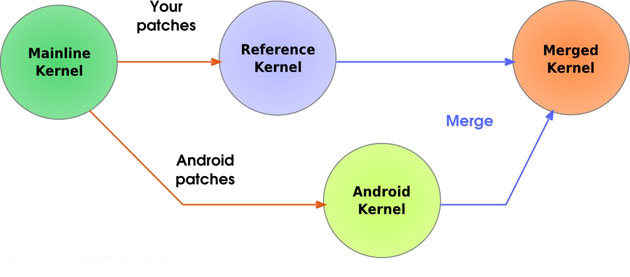
\includegraphics[scale=0.6]{kernel.png}
 
 \tiny Source: \url{http://eecatalog.com/embeddedlinux/2011/08/23/from-zero-to-boot-porting-android-to-your-arm-platform/}
\end{frame}


\begin{frame}{My custom Android kernels}
 \begin{itemize}
  \item Some are based from AOSP (Android Open Source Project) kernels - original source are from Google's git
  \item Some are based from CM (AOSP + Code Aurora Forum (CAF) commits)
  \item Some are based from other custom kernels which are based from two sources above
 \end{itemize}

\end{frame}

\begin{frame}
 \begin{itemize}
  \item I developed my custom kernels for two devices
  \begin{itemize}
   \item Nexus 4 (codename: Mako)
   \item \pause Nexus 5 (codename: Hammerhead) 
   \begin{itemize}
    \item \pause After I sold my Mako :)
   \end{itemize}

  \end{itemize}

 \end{itemize}

\end{frame}


\begin{frame}{Why use custom kernel}
 
 Customization,add-on features:

 \begin{itemize}
  \item \pause Sound patch (for e.g: Faux sound patch)
  \item \pause Allow DoubleTaptoWake(DT2W) or Sweep2Wake, Sweep2Sleep (S2W,S2S) features
  \item \pause Allow many more CPU governors to be used
  \item \pause Allow under/overvolting
  \item \pause Allow number of online/offline CPUs using many methods
  \item \pause Allow many more TCP congestion methods
 \end{itemize}
  
\end{frame}

\begin{frame}{Skillsets for kernel modifying/developing}
\begin{itemize}
 \item Git knowledge
 \begin{itemize}
  \item Knows at least how to clone, pull, push
  \item Then reading git log.. (i'm using --pretty option)
  \item Creating branch, reset to certain checkpoint/offset.. resetting everything (git reset --hard)
 \end{itemize}

 
\end{itemize}

 
\end{frame}


\begin{frame}[fragile]{Git cloning the source}
 \tiny{\begin{verbatim}
najmi@quds:~$ git clone https://android.googlesource.com/kernel/msm -b android-msm-hammerhead-3.4-l-preview
Cloning into 'msm'...
remote: Sending approximately 953.94 MiB ...
remote: Finding sources: 100% (3604873/3604873)
Receiving objects:   0% (14589/3604873), 4.63 MiB | 656.00 KiB/s
 \end{verbatim}}
\end{frame}

\begin{frame}[fragile]
\tiny
\begin{Verbatim}[commandchars=\\\{\}]
najmi@quds:\PYZti{}/cempaka\PYZhy{}kernel\PY{n+nv}{\PYZdl{} }git log \PYZhy{}\PYZhy{}pretty\PY{o}{=}format:
\PY{l+s+s1}{\PYZsq{}\PYZpc{}Cred\PYZpc{}h\PYZpc{}Creset \PYZhy{}\PYZpc{}C(yellow)\PYZpc{}d\PYZpc{}Creset \PYZpc{}s \PYZpc{}Cgreen(\PYZpc{}cr)
\PYZpc{}C(bold blue)\PYZlt{}\PYZpc{}an\PYZgt{}\PYZpc{}Creset
\PYZsq{}} \PYZhy{}\PYZhy{}abbrev\PYZhy{}commit
ba22633 \PYZhy{} \PY{o}{(}HEAD, origin/cempaka\PYZhy{}stable, cempaka\PYZhy{}stable\PY{o}{)}
Cempaka v2.5 \PY{o}{(}11 days ago\PY{o}{)} \PYZlt{}Muhammad Najmi Ahmad Zabidi\PYZgt{}
acaaeea \PYZhy{} Merge branch \PY{l+s+s1}{\PYZsq{}ElementalX\PYZhy{}1.00\PYZhy{}cm\PYZsq{}} of
https://github.com/flar2/ElementalX\PYZhy{}N5 into cempaka\PYZhy{}stable \PY{o}{(}11 days ago\PY{o}{)} \PYZlt{}Muhammad Najmi Ahmad Zabidi\PYZgt{}
039a263 \PYZhy{} \PY{o}{(}elementalx/ElementalX\PYZhy{}1.00\PYZhy{}cm\PY{o}{)} Merge branch \PY{l+s+s1}{\PYZsq{}ElementalX\PYZhy{}1.00
\PYZsq{}} into ElementalX\PYZhy{}1.00\PYZhy{}cm 
\PY{o}{(}12 days ago\PY{o}{)} \PYZlt{}flar2\PYZgt{}
cb7e4f0 \PYZhy{} \PY{o}{(}elementalx/ElementalX\PYZhy{}1.00\PY{o}{)} update defconfig \PY{o}{(}12 days ago\PY{o}{)} \PYZlt{}flar2\PYZgt{}
753de48 \PYZhy{} msm\PYZhy{}sleeper: use ex\PYZus{}max\PYZus{}freq \PY{o}{(}12 days ago\PY{o}{)} \PYZlt{}flar2\PYZgt{}
c5cc9d2 \PYZhy{} Merge branch \PY{l+s+s1}{\PYZsq{}ElementalX\PYZhy{}1.00\PYZsq{}} into
ElementalX\PYZhy{}1.00\PYZhy{}cm \PY{o}{(}2 weeks ago\PY{o}{)} \PYZlt{}flar2\PYZgt{}
8438630 \PYZhy{} vibrator: change permissions again \PY{o}{(}2 weeks ago\PY{o}{)} \PYZlt{}flar2\PYZgt{}
e51fa2d \PYZhy{} Revert \PY{l+s+s2}{\PYZdq{}vibrator: change sysfs permissions\PYZdq{}} \PY{o}{(}2 weeks ago\PY{o}{)} \PYZlt{}flar2\PYZgt{}
9949aff \PYZhy{} Merge branch \PY{l+s+s1}{\PYZsq{}ElementalX\PYZhy{}1.00\PYZsq{}} into ElementalX\PYZhy{}1.00\PYZhy{}cm \PY{o}{(}3 weeks ago\PY{o}{)} \PYZlt{}flar2\PYZgt{}
cbee9fe \PYZhy{} update defconfig \PY{o}{(}3 weeks ago\PY{o}{)} \PYZlt{}flar2\PYZgt{}
\end{Verbatim}
\end{frame}

\begin{frame}
 \begin{itemize}
  \item Most of the developers' works are hosted on github
  \item Some use sourceforge's git and bitbucket's 
  \item I prefer github because I am familiar with it
 \end{itemize}

\end{frame}


%\begin{frame}
%\tikzstyle{decision} = [diamond, draw, fill=blue!20, 
%    text width=4.5em, text badly centered, node distance=3cm, inner sep=0pt]
%\tikzstyle{block} = [rectangle, draw, fill=red!80!green!80!blue!80, 
%    text width=5em, text centered, rounded corners, minimum height=4em]
%\tikzstyle{line} = [draw, -latex']
%\tikzstyle{cloud} = [draw, ellipse,fill=red!20, node distance=3cm,
%    minimum height=2em]
%    \tiny
%\begin{tikzpicture}[node distance = 2cm, auto]
    % Place nodes
  
  %\node [block] (AOSP) {AOSP kernel};
  % \node [cloud, left of=init] (expert) {expert};
  % \node [cloud, right of=init] (system) {system};
   % \node [block,  fill=red!50!green!80!blue!100,  below right 2cm of=AOSP, node distance=4cm] (franco) {Franco gombak kernel};
   % \node [block,  fill=red!50!green!80!blue!100,  below of=AOSP, node distance=2cm] (ampang) {Ampang kernel};
   % \node [block,  fill=red!50!green!80!blue!100,  below right of=AOSP, node distance=2cm] (hellscore) {Hellscore kernel};
   % \node [block,  fill=red!50!green!80!blue!100,  below left of=AOSP, node distance=2cm] (semaphore) {Semaphore kernel};
   % \node [block, fill=red!80!green!80!blue!100,  below of =hellscore, node distance=2cm] (zulfa) {Zulfa kernel};
   % \node [block, fill=red!80!green!80!blue!100,  below of=semaphore, node distance=2cm] (pandan) {Pandan kernel};
   %\node [block, below of=identify] (evaluate) {evaluate candidate models};
    %node [block, left of=evaluate, node distance=3cm] (update) {update model};
   %\node [decision, below of=evaluate] (decide) {is best candidate better?};
   %\node [block, below of=decide, node distance=3cm] (stop) {stop};
    % Draw edges
   % \path [line] (AOSP) -- (ampang);
   % \path [line] (AOSP) -- (hellscore);
   % \path [line] (AOSP) -- (semaphore);
   % \path [line] (AOSP) -- (franco);
   % \path [line] (hellscore) -- (zulfa);
   % \path [line] (semaphore) -- (pandan);
    %path [line] (identify) -- (evaluate);
    %path [line] (evaluate) -- (decide);
    %path [line] (decide) -| node [near start] {yes} (update);
    %path [line] (update) |- (identify);
    %path [line] (decide) -- node {no}(stop);
    %path [line,dashed] (expert) -- (init);
    %path [line,dashed] (system) -- (init);
    %path [line,dashed] (system) |- (evaluate);
%\end{tikzpicture}
%\end{frame}

\begin{frame}{My kernel projects for Nexus 4/Mako}
 \tikzset{
  basic/.style  = {draw, text width=3cm, drop shadow, rectangle},%font=\sffamily, rectangle},
  root/.style   = {basic, rounded corners=1pt, thin, align=center,
                   fill=red!40!blue!80!green!100},
  level 2/.style = {basic, rounded corners=1pt, thin,align=center, fill=red!30!blue!50!green!100,
                   text width=8em},
  level 3/.style = {basic, thin, align=left, fill=red!70!blue!90!green!100,text width=8em}
}

\begin{tikzpicture}[
  level 1/.style={sibling distance=23mm},
  edge from parent/.style={->,draw},
  >=latex]
\tiny
% root of the the initial tree, level 1
\node[root] {Kernel Sources}
% The first level, as children of the initial tree
  child {node[level 2] (c1) {Semaphore Kernel}}
  child {node[level 2] (c2) {Hellscore Kernel}}
  child {node[level 2] (c3) {Ampang Kernel}}  
  child {node[level 2] (c4) {Franco Kernel}}
  child {node[level 2, fill=red!90!blue!90!green!90] (c5) {Aufa Kernel (CM based kernel)}} ; 
% The second level, relatively positioned nodes
\begin{scope}[every node/.style={level 3}]
\node [below of = c1, xshift=15pt] (c11) {Pandan Kernel};
\node [below of = c2, xshift=15pt] (c21) {Zulfa Kernel};
\node [below of = c4, xshift=15pt] (c41) {Franco Gombak Kernel};


\end{scope}

% lines from each level 1 node to every one of its "children"
%\foreach \value in {1,2,3}
\foreach \value in {1}
  \draw[->] (c1.205) |- (c1\value.west);

%\foreach \value in {1,...,4}
\foreach \value in {1}
  \draw[->] (c2.195) |- (c2\value.west);

\foreach \value in {1}
  \draw[->] (c4.195) |- (c4\value.west);
  

  
\end{tikzpicture}
\end{frame}



\begin{frame}{My kernel projects for Nexus 5/Hammerhead}
 \tikzset{
  basic/.style  = {draw, text width=3cm, drop shadow, rectangle},%font=\sffamily, rectangle},
  root/.style   = {basic, rounded corners=1pt, thin, align=center,
                   fill=red!40!blue!80!green!100},
  level 2/.style = {basic, rounded corners=1pt, thin,align=center, fill=red!30!blue!50!green!100,
                   text width=10em},
  level 3/.style = {basic, thin, align=left, fill=red!70!blue!90!green!100,text width=10em}
}

\begin{tikzpicture}[
  level 1/.style={sibling distance=30mm},
  edge from parent/.style={->,draw},
  >=latex]
\tiny
% root of the the initial tree, level 1
\node[root] {Kernel Sources}
% The first level, as children of the initial tree
  child {node[level 2] (c1) {ElementalX}}
  child {node[level 2] (c2) {CodeBlue}}
  child {node[level 2] (c3) {Jerung Kernel}}
  child {node[level 2, fill=red!90!blue!90!green!90] (c4) {Lekiu Kernel (for L preview)}} 
  ; 
% The second level, relatively positioned nodes
\begin{scope}[every node/.style={level 3}]
\node [below of = c1, xshift=15pt] (c11) {Cempaka Kernel};
\node [below of = c2, xshift=15pt] (c21) {Blue Kelisa Kernel};

\end{scope}

% lines from each level 1 node to every one of its "children"
%\foreach \value in {1,2,3}
\foreach \value in {1}
  \draw[->] (c1.190) |- (c1\value.west);

%\foreach \value in {1,...,4}
\foreach \value in {1}
  \draw[->] (c2.190) |- (c2\value.west);

%\foreach \value in {1}
%  \draw[->] (c4.195) |- (c4\value.west);
  

  
\end{tikzpicture}
\end{frame}
 

\end{document}



